\section{Preconditioners}
\label{sec:preconditioners}
The convergence of any iterative solver is highly dependent on the properties of the matrix $A$ (e.g. eigenvalues, singular values, etc. - depending on the solving technique). Preconditioning is a method of transforming the linear system in such a way, that these properties of the matrix are improved and faster convergence can be achieved. According to \cite{golub_matrix_2013}, any Krylov method used to solve the system $Ax=b$ will converge more rapidly if $A \in \realx{n}$ is "close to the identity matrix $I$". This basic concept (and its advantages) are illustrated in Figure~\hyperref[fig:preconditioning]{\ref{fig:preconditioning}}. For example, for a symmetric positive definite matrix $A$ with $A \approx I +\Delta A$ and $rank(\Delta A)=c \ll n$, the CG method should produce a good approximation to the actual solution in about $c$ iterations.

\begin{figure}
\centering
\begin{subfigure}{.5\textwidth}
  \centering
  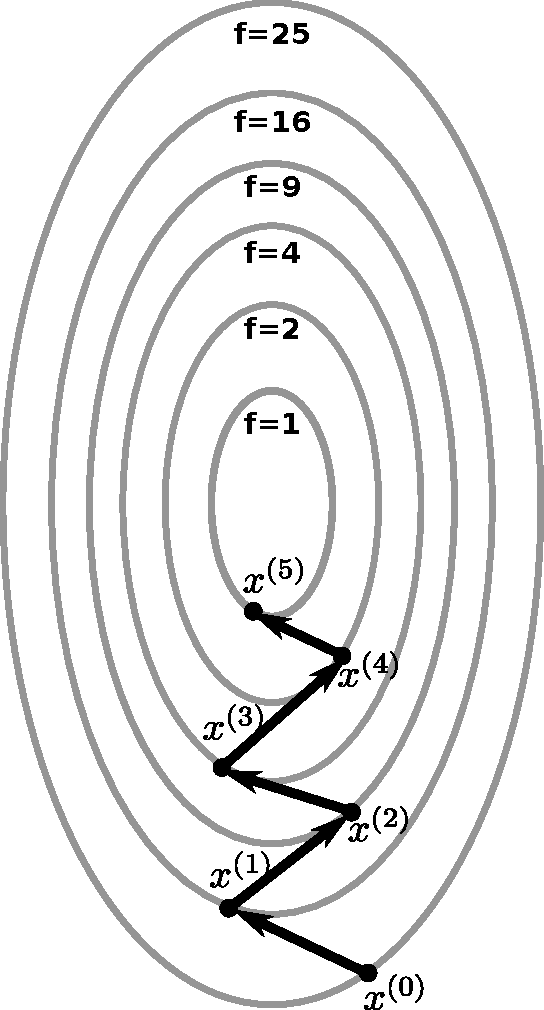
\includegraphics[width=0.685\linewidth]{figures/no_preconditioner.pdf}
  \caption{Original Linear System}
  \label{fig:no_preconditioner}
\end{subfigure}%
\begin{subfigure}{.5\textwidth}
  \centering
  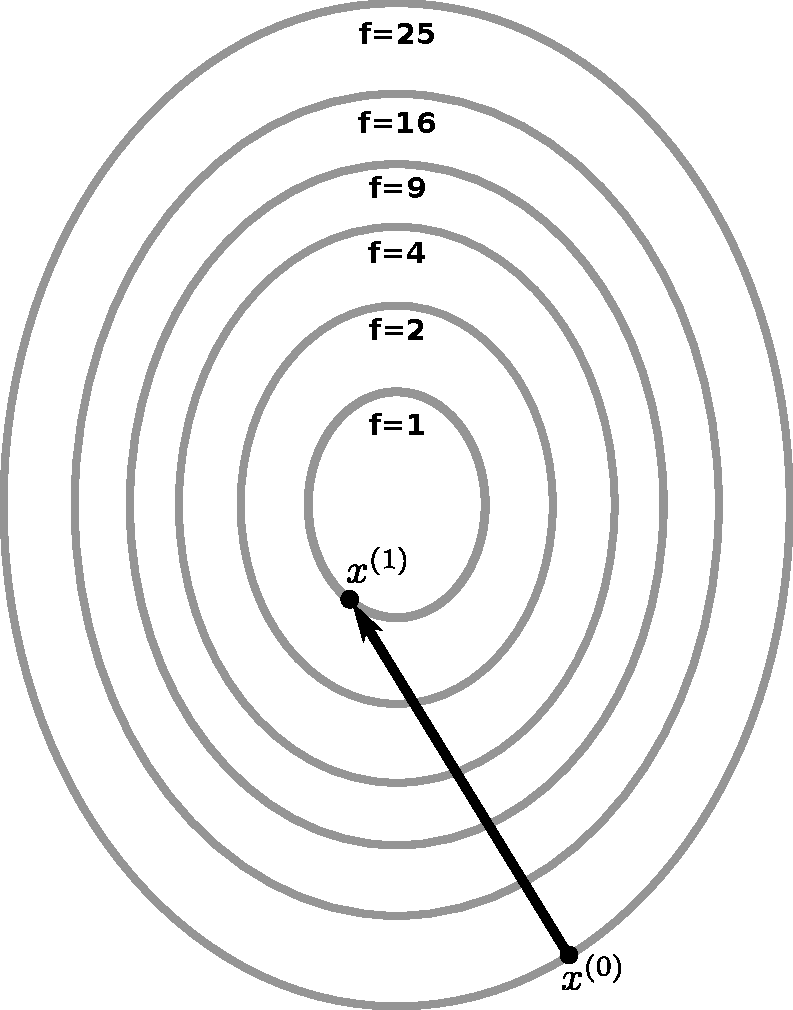
\includegraphics[width=\linewidth]{figures/preconditioner.pdf}
  \caption{Preconditioned Linear System}
  \label{fig:preconditioner}
\end{subfigure}
\caption{Illustrating the benefit of applying a preconditioner. The original system needs 5 iterations to obtain a good solution, while the preconditioned system only needs one.}
\label{fig:preconditioning}
\end{figure}

Generally, the solution to the linear system defined above can be rewritten for any non-singular matrix $M \in \realx{n}$ to form the following system:
\begin{equation}
\label{eqn:preconditioner}
    \inverse
    {M}Ax = \inverse{M}b
\end{equation}

\noindent This system has the same solution as the original one, but the convergence properties now depend on $\inverse{M}A$ instead of just $A$. Thus, if this \textit{preconditioner} $M$ is selected carefully, the problem might be solvable in less steps by any iterative method. It is noteworthy that Equation~\hyperref[eqn:preconditioner]{\ref{eqn:preconditioner}} is not the only possible formulation of such a preconditioned system. Defining $M=M_LM_R$ leads to the more general formulation:
\begin{equation}
    \inverse{M_L}A\inverse{M_R}y = \inverse{M_L}b\;\; \text{ with }\;\; M_Rx=y
\end{equation}

\noindent In this context $M_L$ is referred to as a \textit{left} preconditioner (similar to Equation~\hyperref[eqn:preconditioner]{\ref{eqn:preconditioner}}), while $M_R$ is called a \textit{right} preconditioner and both approaches (or the combination of them) are used in practice. However, for a matrix $M$ to be suitable as a preconditioner for the system $Ax=b$, it must have the following properties (as listed in \cite{golub_matrix_2013}):
\begin{itemize}
    \item It must capture the essence of the matrix $A$ (or worded differently, $\inverse{M}$ must capture the essence of $\inverse{A}$), because if $M \approx A$, then $\inverse{M_L}A\inverse{M_R} \approx I$ and convergence becomes fast.
    \item It must be easy to solve linear systems that involve $M_L$ and $M_R$, since iterative solvers usually execute a $\inverse{M_L}A\inverse{M_R}$-times vector operation.
\end{itemize}

\noindent The last criterion hints at the trade-off involved when using a preconditioner, which lies in the additional overhead introduced per iteration versus the number of iterations necessary. Citerion one, on the other hand, basically implies that the error matrix $E=A-M$ should be either small in norm or low in rank.

In this context, it is time to re-visit the stationary iterative solvers (discussed in Section~\hyperref[sec:stationary_methods]{\ref{sec:stationary_methods}}), based on the splitting of the matrix $A$ into $A=M-N$. The iteration in this case takes the form of:
\begin{equation}
    \iter[i+1]{x}\inverse{M}N\iter[k]{x}+\inverse{M}b
\end{equation}

\noindent By defining
\begin{equation}
    G=\inverse{M}N=\inverse{M}(M-A)=I-\inverse{M}A\;\; \text{ and } \;\; f=\inverse{M}b
\end{equation}

\noindent the iteration $\iter[k+1]{x}=G\iter{x}+f$ can be seen as a technique to solve:
\begin{equation}
    (I-G)x = f
\end{equation}

\noindent Which can be rewritten as:
\begin{equation}
    {M}Ax = \inverse{M}b
\end{equation}

\noindent From this, it becomes obvious that stationary iterative solvers are equivalent to a fixed-point iteration on a preconditioned system. Consequently, the splittings used for the matrix $M$ in Jacobi (diagonal part), Gauss-Seidel or SOR (lower triangular part) methods are readily available preconditioners. An important observation is that in the case of symmetric Gauss-Seidel (or SOR), the preconditioner takes the form $M=LU$ (note that this is not based on Gaussian elimination and thus easily attainable) where $L$ is unit lower triangular and $U$ is upper triangular. Hence, the calculation of $\inverse{M}x=y$ can be done with two triangular solves, only involving a complexity of $\mathcal{O}(n^2)$.

\subsection{Approximate Inverse Preconditioners}
\label{sec:inverse_preconditioners}
As mentioned earlier, the condition for the preconditioner $M \approx A$ can be also rewritten as $\inverse{M} \approx \inverse{A}$. Capturing the essence, in this case can be interpreted as finding $\inverse{M}$ so that:
\begin{equation}
    \norm{A\inverse{M}-I}_2 = \text{ minimum}
\end{equation}

\noindent This concept summarizes the main idea behind an approximate inverse preconditioner. However, to assure that the calculations remain computationally feasible, it is necessary to define some restrictions on the structure of the inverse, with the most general case being sparsity. In order to make this concept more precise, consider the $sparse()$ operator as defined by \cite{golub_matrix_2013}. For any matrix $T \in \realx{n}$, $sparse(T) \in \realx{n}$ this operator gives:
\begin{equation}
    \left[ sparse(T)\right]_{i,j} =\begin{cases}
      1 & \text{if } t_{i,j} \neq 0\\
      0 & \text{otherwise }\\
    \end{cases}  
\end{equation}

\noindent Given any matrix $Z \in \realx{n}$ with a manageable sparsity pattern (i.e. enough zeros for a fast computation), the goal is to obtain a matrix $T$ (having the same sparsity pattern) such that:
\begin{equation}
    \underset{sparse(T)=Z}{min} \norm{AT-I}_2
\end{equation}

\noindent The preconditioner is then specified through its inverse: $\inverse{M}=T$ and a system of the form $Mz=y$ can be solved via the matrix-vector multiplication $z=Ty$.

Another method to get a good estimate of the inverse of the matrix $A$ is via polynomial approximation. Given a splitting of the form $A=M-N$ and $G=\inverse{M}N$, where $\rho(G)<1$ it follows that:
\begin{equation}
    \inverse{A}=\inverse{(I-G)}\inverse{M} = \left(\sum_{k=1}^{\infty}G^k\right)\inverse{M}
\end{equation}

\noindent As such, an approximation of $\inverse{A}$ can be obtained by simply truncating this infinite series:
\begin{equation}
    \inverse{A} \approx \left(\sum_{k=0}^{m}G^k\right)\inverse{M}
\end{equation}

\noindent Consequently, a solution to the system $Mz=y$ cn be obtained from:
\begin{equation}
    z = (I+G+G^2+\dots+G^m)\inverse{M}y
\end{equation}

\noindent Furthermore, this solution can be obtained in a very simple way requiring $m$ steps of the iteration outlined in Algorithm~\hyperref[alg:poly_preconditioner]{\ref{alg:poly_preconditioner}}. Thus the actual preconditioner for this system becomes $\Tilde{M}$ given by:
\begin{equation}
    \inverse{\Tilde{M}}=p(\inverse{M}A)\inverse{M}
\end{equation}

\begin{algorithm}[h]
  \caption{Polynomial Preconditioner - Solve}
  \label{alg:poly_preconditioner}
  \SetAlgoLined
  \DontPrintSemicolon
  \KwIn{matrices $M,N \in \mathbb{R}^{n \times n}$, vector $y \in \mathbb{R}^{n}$}
  \KwOut{approximate solution $\iter[m]{z}$ to the system $Mz=y$\\
  \hrulealg}
  $\iter[0]{z} = 0$ \\
  \For{$k = 1$ \KwTo $m$} {
    $\iter{z} = \inverse{M}N\iter[k-1]{z}+y$ \\
  }
\end{algorithm}

\noindent In this setting, $p$ is a polynomial and $M$ itself is a preconditioner (e.g. Jacobi preconditioner). It should be mentioned that the method introduced here is the most basic form of a polynomial preconditioner and there are many, more sophisticated way to obtain a good approximation of $\inverse{A}$ (see \cite{golub_matrix_2013}).


\subsection{Incomplete Factorization Preconditioners}
\label{sec:incomplete_preconditioners}

Since a preconditioner works best if it is close to the original matrix $A$, it is natural to consider the usage of matrix decompositions for this purpose. However, general factorizations such as LU or QR involve a runtime complexity of $\mathcal{O}(n^3)$, which is equal to the cost of a direct solver. Since this is too expensive for the purpose of preconditioning, the key idea of incomplete factorizations is to calculate an approximate decomposition at much lower cost, while still being able to represent the original matrix. Those methods have been originally developed in the context of sparse linear systems, but can be generalized to be applicable for dense matrices as well.

On of the most popular methods is the incomplete LU (ILU) factorization (or incomplete Cholesky for the symmetric case). It has been developed as a method to reduce the fill-in (replacing zero entries with non-zero entries) that usually happens during the factorization of a spares matrix by dropping some elements in predetermined (non-diagonal) positions. The sparsity pattern of the resulting decomposition is typically chosen in advance, based on the original matrix $A$. Therefore, a zero pattern set $P$ needs to be defined such that:
\begin{equation}
    P \subset \{(i,j)|i \neq j; 1 \leq i,j\leq n\}
\end{equation}

\noindent It is important to note that this set can not include the diagonal, as this would lead to a breakdown of the method. The pseudo-code to obtain such an ILU factorization for any sparsity Pattern $P$ (often, this set is chosen to be identical to the sparsity pattern of the original matrix $sparse(LU)=A$) is provided in Algorithm~\hyperref[alg:ilu]{\ref{alg:ilu}} (adapted from \cite{saad_iterative_2003}). 

\begin{algorithm}[h]
  \caption{Incomplete LU}
  \label{alg:ilu}
  \SetAlgoLined
  \KwIn{non-singular matrix $A \in \mathbb{R}^{n \times n}$, sparsity pattern $P$}
  \KwOut{ Incomplete LU factorization stored in matrix $B \in \mathbb{R}^{n \times n}$ \\
  \hrulealg}
  $B=A$ \\
  \ForEach{$(i,j)\in P$}{$b_{i,j}=0$\\}
  \For{$k = 1$ \KwTo $n-1$} {
    \For{$i = k+1$ \KwTo $n$} {
      \If{$(i,k) \notin P$}
      {$b_{i,k}=b_{i,k}/b_{k,k}$}
      \For{$j = k+1$ \KwTo $n$} {
      \If{$(i,j) \notin P$}
        {$b_{i,j}=b_{i,j}-b_{i,k}*b_{k,j}$}
      }
    }
  }
\end{algorithm}

As an alternative to a position based sparsity pattern, it is also possible to compute a thresholded ILU factorization (often denoted as ILUT), replacing values that are below a pre-defined tolerance with zeros. As this allows for a certain amount of fill-in, depending on the threshold parameter, more accurate approximations to the original matrix $A$ can be achieved. However, this is only favourable if the original matrix already features a sparse structure and can thus only be employed to the general case if a sparsity pattern has been enforced beforehand.

Another, relatively new addition to the field of preconditioners are low-rank approximations (see \cite{markovsky_low_2011}). Instead of obtaining a fast, approximate decomposition by enforcing a sparsity pattern, they aim to accomplish the same goal by reducing the dimensions of the matrix. A rank $k$ approximation can thus be defined by selecting two matrices $U$ and $V$ as follows:
\begin{equation}
    A \in \realx{n}\text{,}\:\; U \in \realx[n]{k}\;\; \text{ and }\;\; V \in \realx[k]{n}
    \text{such that }\;\ A \approx UV
\end{equation}

\noindent The most simple and accurate example of such a factorization would be a truncated singular value decomposition (SVD) consisting of a full SVD $A=USV$ that is truncated to its $k$ first terms (as depicted in Figure~\hyperref[fig:svd]{\ref{fig:svd}}). While this procedure would lead to the smallest possible error according to the Eckhart-Young theorem \cite{eckart_approximation_1936}, it is prohibitively expensive and other techniques such as adaptive cross approximation (ACA) \cite{rjasanow_adaptive_2000} or randomized approaches \cite{martinsson_randomized_2019} are used. However, because $k \ll n$ is required for this method to be feasible, it is applicable only to matrices that exhibit such a low-rank property and its practical usage is limited to certain applications (see \cite{higham_new_2019} for an example).

\begin{figure}[h]
    \centering
    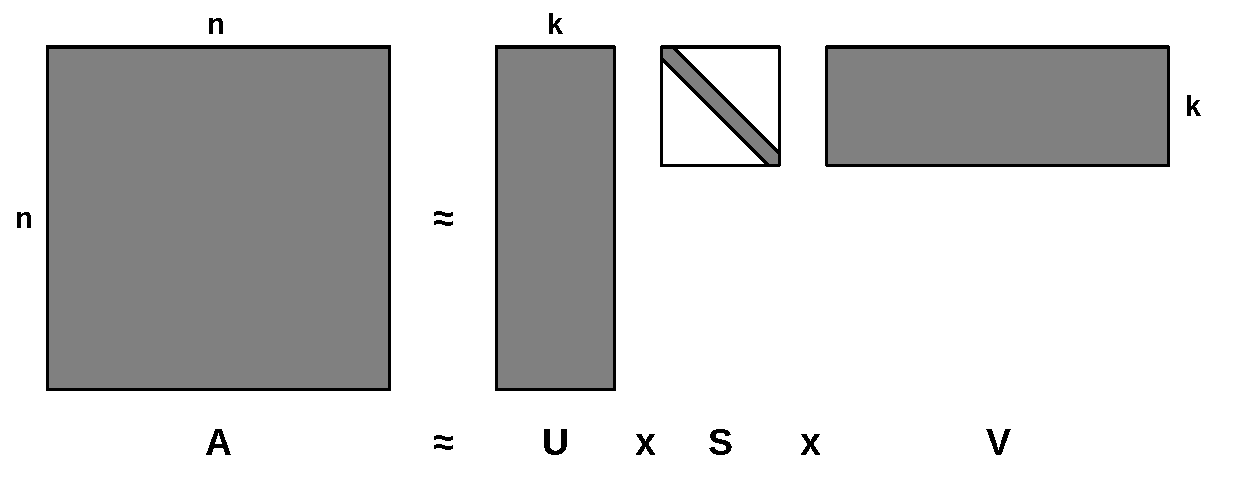
\includegraphics[width=0.7\linewidth]{figures/SVD.pdf}
    \caption{Truncated SVD of a matrix $A \in \realx{n}$}.
    \label{fig:svd}
\end{figure}

Fortunately, even if a matrix is not low-rank by itself, it might exhibit a rank structure, that can be exploited by a number of rank-structure formats such as $\mathcal{H}$-matrices (these formats will be introduced and discussed in Chapter~\hyperref[chap:hierarchical_matrices]{\ref{chap:hierarchical_matrices}}.
In general, those formats allow for an approximate LU factorization to be calculated in $\mathcal{O}(n \;log(n))$ or even $\mathcal{O}(n)$, making them most suitable for a preconditioner. Despite those favourable properties, the usage of this techniques has been mostly limited to special types of matrices (usually arising from the discretisation of elliptic partial differential equations - see \cite{gatto_preconditioner_2015} \& \cite{gatto_efficient_2017}). Examining whether or not they can be beneficial for the general case as well, is the purpose of this research.